%!TEX root = ms.tex
\section{Best orthogonalized subset selection (BOSS)}
\label{sec:boss}
With a general $X$, BS is not computationally feasible for large problems. In this section, we propose a LS-based subset selection method BOSS that has computational cost of the same order as a multiple regression on all of the predictors. 

\subsection{The method and its computational cost}
\label{sec:boss_alg}
The detailed implementation process of BOSS is described in Algorithm \ref{alg:boss}. The main steps can be summarized as follows: 1) order and orthogonalize the predictors, 2) perform BS on the set of orthogonal predictors, 3) transform the coefficients back to the original space, and 4) use a selection rule such as AICc-hdf to choose the single subset.

% main algorithm
\begin{algorithm}
	\caption{Best Orthogonalized Subset Selection (BOSS)}\label{alg:boss}
	\begin{enumerate}[label=\arabic*.]
		\item Standardize $y$ and the columns of $X$ to have mean $0$, and denote the means as $\bar{X}$ and $\bar{y}$.
		%\item Denote $S_k$ as the set of predictors that are active at step $k$ and let $S={1,\cdots, p}$.

		\textbf{Order and orthogonalize the predictors:}

		\item From the $p$ predictors, select the one that has the largest marginal correlation with the response $y$,  and denote it as $X_{S_1}$. Standardize $X_{S_1}$ to have unit $l_2$ norm and denote it as $Q_{S_1}$. Calculate $R_{S_1}$ such that $X_{S_1} = Q_{S_1} R_{S_1}$. Let $S=\{1,\cdots, p\}$. Initialize vectors $\text{resid}_j=X_j$ where $j=1,\cdots,p$.
		\item For $k=2,\cdots,p$:
		\begin{enumerate}[label=\alph*.]
			\item For each of the $p-k+1$ predictors $X_j$ in $X_{S \setminus S_{k-1} }$, calculate its partial correlations with the response $y$ conditioning on $Q_{S_{k-1}}$. 
			\iffalse
			\begin{enumerate}[label=a\arabic*.]
				\item Regress $y$ on $q$, augment $Z$ with the coefficient $z$. Set $\text{resid1} = \text{resid1} - zq$.
			\end{enumerate}
			\fi
			%\begin{enumerate}[resume*,label=a\arabic*.]
			\begin{enumerate}[label=a\arabic*.]
				%\item Regress $x_j$ on $q$, call the coefficient $r$. Set $\text{resid2}_j = \text{resid2}_j - rq$.
				%\item Calculate the correlation between resid1 and $\text{resid2}_j$.
				\item Regress $X_j$ on $Q_{S_{k-1} \setminus S_{k-2}}$ ($S_{k-2}=\emptyset$ if $k=2$), and denote the estimated coefficient as $r$. Update $\text{resid}_j = \text{resid}_j - r Q_{S_{k-1} \setminus S_{k-2}}$.
				\item Calculate the correlation between y and $\text{resid}_j$.
			\end{enumerate}
			\item Select the predictor that has the largest partial correlation in magnitude, augment $S_{k-1}$ with this predictor and call it $S_{k}$.
			\item Update $Q_{S_{k-1}}$ and $R_{S_{k-1}}$ given the newly added column $X_{S_k \setminus S_{k-1}}$, and call them $Q_{S_k}$ and $R_{S_k}$. The update is based on the modified Gram-Schmidt algorithm as discussed in \citet{hammarling2008updating}.
		\end{enumerate}
		
		\textbf{BS on the orthogonalized predictors $Q_{S_{p}}$:}

		\item Calculate $\tilde{\gamma}_j (k_Q)= z_j \mathbbm{1}(|z_j| \ge |z_{(k_Q)}|)$, i.e. the $j$-th component of coefficient vector for subset size $k_Q$, where $z=Q_{S_p}^T y$ and $z_{(k_Q)}$ is the $k$-th largest entry in absolute values. Let $\tilde{\gamma} = [\tilde{\gamma} (0) \tilde{\gamma} (1) \cdots \tilde{\gamma} (p)]$.
		
		\textbf{Transform back to the original space:}

		\item Project $\tilde{\gamma}$, a $p \times (p+1)$ matrix, to the original space of $X_{S_p}$, i.e. back solving $R \tilde{B} = \tilde{\gamma}$, and re-order the rows of $\tilde{B}$ to their correspondences in $X$, i.e. $\hat{B} = O \tilde{B}$ where $O$ represents the ordering matrix s.t. $X_{S_p}=XO$. The intercept vector is $\hat{B}_0 = \bar{y} \mathbbm{1} - \hat{B}^T \bar{X}$. 

		\textbf{Select the subset:}

		\item Select the subset using AICc-hdf, where hdf is calculated via Algorithm \ref{alg:hdf}, by inputting $(Q_{S_p},y)$. The inclusion of an intercept term implies that hdf$(k_Q)$ is increased by $1$.
	\end{enumerate}
\end{algorithm}


As can be seen in what follows, the computation of BOSS has an overall cost of $O(np^2)$, the same cost as OLS on all $p$ predictors and lasso. For step $k$, we have a set of ordered predictors $X_{S_{k-1}}$ and its orthogonal basis $Q_{S_{k-1}}$. From the remaining $p-k+1$ predictors, we choose the one that has the largest correlation with $y$ conditioning on $Q_{S_{k-1}}$, that is the correlation between $y$ and the residual from regressing a candidate predictor on $Q_{S_{k-1}}$. The regression part costs $O(n)$ since we maintain the regression result, e.g. estimated coefficients and residual, in the previous steps, and only need to perform a simple linear regression upon the predictor joined in step $k-1$, i.e. the last column in $Q_{S_{k-1}}$. Repeating the above step for all $p-k+1$ predictors costs $O(n(p-k+1))$. We then update the QR decomposition, by adding the chosen predictor as a new column, which costs $O(n(p-k))$ via the modified Gram-Schmidt algorithm as discussed in \citet{hammarling2008updating}. Therefore, we end up with an ordered set of predictors $X_{S_p}$ and its corresponding QR decomposition $Q_{S_p}$ and $R_{S_p}$. We regress $y$ upon $Q_{S_p}$ which costs $O(np)$, and denote the coefficient vector as $z$. BOSS then performs BS on $Q_{S_p}$, which is a ranking of predictors based on their magnitudes of corresponding element in $z$, and the cost is $O(p\log(p))$. Once we have the solution path of BOSS, we then apply AICc-hdf to choose the single subset size (denoted as $k_Q$), where hdf is calculated via Algorithm \ref{alg:hdf} by inputting $Q_{S_p}$. The entire BOSS-AICc-hdf procedure costs $O(np^2)$. 

The ordering of predictors is essential in terms of both getting a sparse solution and a better predictive performance. Consider a sparse true model with only two uncorrelated predictors $X=[X_1,X_2]$, $\beta=[0,1]^T$ and a high SNR. Based on the evidence we see from the previous section, the best model in such a scenario is LS regression on $X_2$. Without the ordering step, the orthogonal basis is $Q=[Q_1,Q_2]$ s.t. $X=QR$, i.e. the predictors are orthogonalized in their physical orders. The one-predictor model ($k_Q=1$) of BS can either be $Q_1$ or $Q_2$, which when transformed back to the space of $X$ do not correspond to LS regression upon $X_2$. The former corresponds to LS estimates upon $X_1$, while the latter is a linear combination of LS estimates upon $X$ and LS estimates upon $X_1$; the former leads to a completely wrong model while the latter results in non-zero coefficients on both predictors. In contrast, if $X_2$ is the first variable orthogonalized, the best subset will be based on that variable alone, the correct choice. Therefore, the ordering step is crucial to both sparsity as well as predictive performance. Note that we show the coefficients of BOSS can be expressed as a linear combination of LS coefficients on subsets of $X$ in Theorem \ref{thm:correspondence} and the proof can be found in the Supplemental Material. 

BS on the set of orthogonalized predictors gives the chance for BOSS to ``look back'' at the predictors that are already stepped in. One may notice that BOSS is similar to forward stepwise regression (FS), which was first introduced in \citet{efroymson1960multiple}. FS orders and orthogonalizes the predictors in the same way as BOSS. It then takes the nested subsets $Q_{S_1}, Q_{S_2}, \cdots, Q_{S_p}$ as the candidate subsets and performs LS regression upon them. Therefore, once a predictor is stepped in, it remains in the subsets of every following step of FS. As we will show in the next section, under certain circumstances, FS can easily overfit, since noise predictors (those with $\beta_j=0$) step in during early steps. However, BOSS revisits the predictors that have already stepped in and allows them to be dropped, resulting in a better predictive performance than FS.

\begin{theorem}[Coefficients of BOSS are a linear combination of LS coefficients on subsets of $X$] 
	Suppose $X$ has full column rank and the columns are already ordered. $X=QR$ where $Q$ is an $n \times p$ matrix with orthonormal columns and $R$ is a $p \times p$ upper-triangular matrix. Let $S_k=\{j_1,j_2,\cdots,j_{k_Q}\}$ denote the support (position of predictors) of the best $k_Q$-predictor model given by BS upon $(Q,y)$, and use $\hat{\gamma}(k_Q)$ ($p$ by $1$) to denote the BS coefficients. The corresponding coefficients in the $X$ space, i.e. $\hat{\beta}(k_Q)$ s.t. $R\hat{\beta}(k_Q)=\hat{\gamma}(k_Q)$, can be expressed as
	\begin{equation*}
	\hat{\beta}(k_Q) = \sum_{j\in S_k} \left(\hat{\alpha}^{(j)} - \hat{\alpha}^{(j-1)}\right),
	\end{equation*}
	where the first $j$ entries in $\hat{\alpha}^{(j)}$ ($p$ by $1$) are LS coefficients of regressing $y$ upon $[X_1,X_2,\cdots,X_j]$ (the first $j$ columns in $X$), and the remaining $p-j$ entries are zero.

	\label{thm:correspondence}
\end{theorem}

\subsection{Numerical justification of using hdf for BOSS}
The hdf is designed for BS on a set of orthogonal predictors. However, before performing BS on the orthogonal basis, BOSS first orders the predictors. This raises the question as to whether hdf is reasonable to use in the selection rules for BOSS. 

Figure \ref{fig:boss_cp_edf_hdf} compares averages of C$_p$-edf and C$_p$-hdf over $1000$ replications for BOSS under various true models. The details of setups for the sparse and dense models can be found in Section \ref{sec:simulation_setup_generalx}, where they correspond to the Sparse-Ex3 and Dense designs, respectively. The correlation between predictors is $\rho=0.5$. We see that by using the sample average to represent the population mean, $E(\text{C}_p\text{-hdf})$ approximates $E(\text{C}_p\text{-edf})$ well in most cases where the latter is also the expected prediction error $E(\text{Err}_\text{SE})$ by definition, and they converge as $k_Q$ approaches $p$. Moreover, both C$_p$-edf and C$_p$-hdf lead to the same average selected subset size, supporting the use of hdf in model selection for BOSS. 

Note that for any general fitting procedure including BOSS, C$_p$ provides an unbiased estimator of the testing error, and for that reason it is used in our discussions about the best-case performance when $\sigma$ is assumed to be known. Unfortunately, as discussed in Section \ref{sec:bs_ic_simulationresults}, using C$_p$ as the selection rule for BS can perform poorly in practice because of the need to estimate $\sigma$, particularly when $p$ is close to $n$. A similar property of using C$_p$ as the selection rule for BOSS will be shown in Section \ref{sec:boss_regu}. Therefore we prefer AICc in feasible versions of selection since it can perform considerably better. 

% {fig:boss_cp_edf_hdf}
\begin{figure}[ht!]
	\centering
	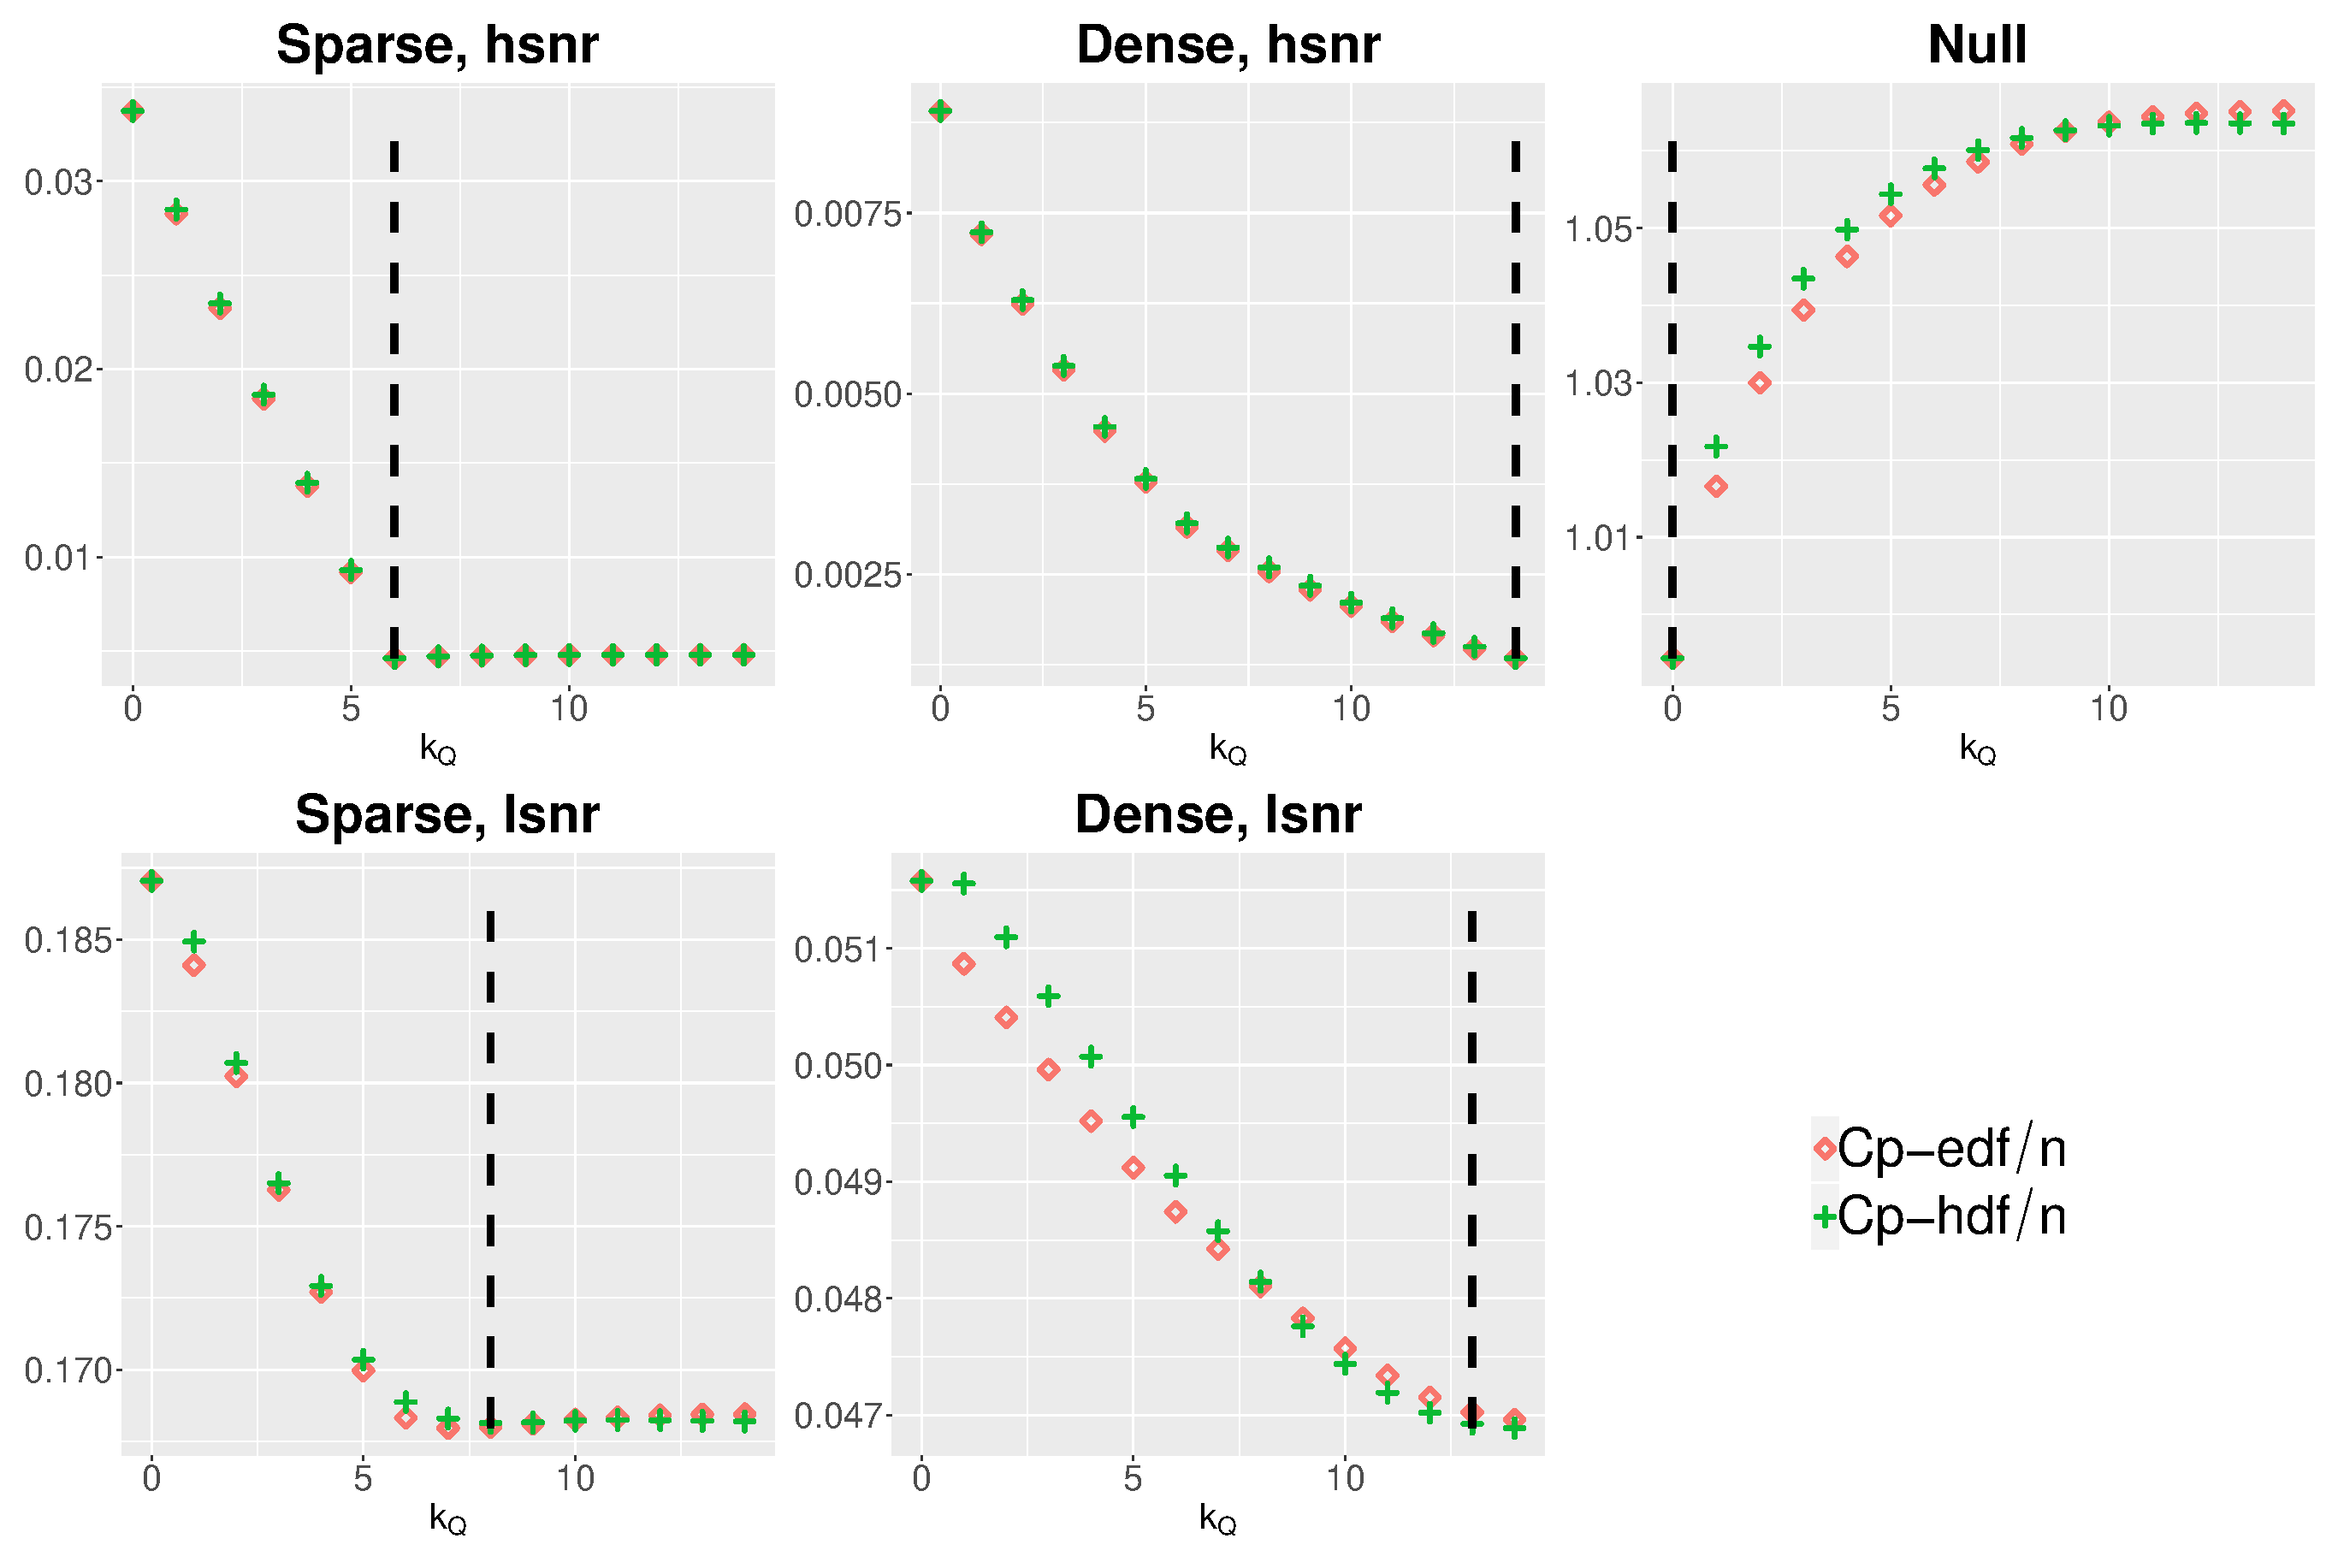
\includegraphics[width=0.9\textwidth]{figures/cp_edf_hdf_boss.eps}
	\caption{Averages of C$_p$-edf and C$_p$-hdf for BOSS over $1000$ replications. Here $X$ is general with $n=200$, $p=14$. Both criteria result in the same average of the selected subset size over the $1000$ replications (rounded to the nearest integer) as denoted by the dashed vertical lines. We assume knowledge of $\mu$ and $\sigma$.}
	\label{fig:boss_cp_edf_hdf}
\end{figure}

\subsection{The performance of BOSS}
We now study the performance of BOSS via simulations. We first show that BOSS can provide a better solution path than FS, and we further compare BOSS with regularization methods. 

\subsubsection{Simulation setups}
\label{sec:simulation_setup_generalx}
We consider a similar setup as in Section \ref{sec:simulation_setup_orthx}, but with a general $X$, where  $x_i\sim \mathcal{N}(0,\Sigma)$, $i=1,\cdots,n$ are independent realizations from a $p$-dimensional multivariate normal distribution with mean zero and covariance matrix $\Sigma=(\sigma_{ij})$. 

The correlation structure and true coefficient vector $\beta$ include the following scenarios:
\begin{itemize}
	\item Sparse-Ex1: \textbf{All of the predictors (both signal and noise) are correlated.} We take $\sigma_{i,j}=\rho^{|i-j|}$ for $i,j\in\{1,\cdots,p\}\times\{1,\cdots,p\}$. As to $\beta$, we have $\beta_j=1$ for $p_0$ equispaced values and $0$ everywhere else. 
	\item Sparse-Ex2: \textbf{Signal predictors are pairwise correlated with opposite effects.} We take $\sigma_{i,j}=\sigma_{j,i}=\rho$ for $1\le i <j \le p_0$. Other off-diagonal elements in $\Sigma$ are zero. For the true coefficient vector, we have $\beta_{2j-1}=1$ and $\beta_{2j}=-1$ for $1\le j \le p_0/2$, and all other $\beta_j=0$ for $j=p_0+1,\cdots,p$.
	\item Sparse-Ex3: \textbf{Signal predictors are pairwise correlated with noise predictors.} We take $\sigma_{i,j}=\sigma_{j,i}=\rho$ for $1\le i \le p_0$ and $j=p_0+i$. Other off-diagonal elements in $\Sigma$ are zero. $\beta=[1_{p_0},0_{p-p_0}]^T$.
	\item Sparse-Ex4: \textbf{Same correlation structure as Sparse-Ex2, but with varying strengths of coefficients.} We have $\beta_j=-\beta_{j+1}$ where $j=2k+1$ and $k=0,1,\cdots,p_0/2-1$. Suppose that $\beta^\prime=[1,5,10]$, then $\beta_j=\beta^\prime_k$ where $k=j (\text{mod} 3)$. 
	\item Dense: \textbf{Same correlation structure as Ex1, but with diminishing strengths of coefficients}. The true coefficient vector has: $\beta_j = \displaystyle (-1)^j \exp(-\frac{j}{\kappa})$, $j=1,\cdots,p$, and here $\kappa=10$.
	%\item Dense-Ex2: \textbf{Same setup as Dense-Ex1, but with slower decay}. Here we take $\kappa=50$.
\end{itemize}
The setup of Sparse-Ex1 is very common in the literature, such as in \citet{Bertsimas2016} and \citet{Hastie2017}. All of the predictors are correlated (when $\rho \ne 0$) where the strength of correlation depends on the physical positions of variables. Sparse-Ex2 is designed such that the pair of correlated predictors, e.g. $(X_1,X_2)$, leads to a good fit (high $R^2$), while either single one of them contribute little to the fitted $R^2$. Sparse-Ex4 is similar to Sparse-Ex2, but has varying strengths of coefficients for the true predictors. In Sparse-Ex3, signal predictors are only correlated with the noise ones. Finally, the dense setup is built on the dense example in Section \ref{sec:simulation_setup_orthx}, by having correlated predictors.

For the sparse examples, we take $p_0=6$. We consider three values of the correlation parameter, $\rho \in [0, 0.5, 0.9]$. Other configuration options, including $n$, $p$, and SNR, are the same as in Section \ref{sec:simulation_setup_orthx}. This implies a total of $360$ different combinations of configuration options. For each configuration, $1000$ replications are estimated and we present the same evaluation measures as introduced in Section \ref{sec:simulation_setup_orthx}. The full set of results can be found in the Supplemental Material.


\subsubsection{The solution paths of BOSS and FS}
Unlike FS, whose candidate subsets are nested, BOSS performs an extra step of BS upon $Q_{S_p}$, which raises the question of whether the extra step brings any benefit. We set aside the selection rule for now, and focus on the solution paths of the two methods. 

Figure \ref{fig:lossratio_fs_boss_k} shows two examples of the average RMSE along the solution paths of BS, FS and BOSS. When the true model is Sparse-Ex3, all three methods provide almost the same solution path. However, for Sparse-Ex4, we see a clear advantage of BOSS over FS in early steps up until about the fifteenth step. Recall that in Sparse-Ex4, there are $p_0=6$ predictors with $\beta_j \ne 0$ that are pairwise correlated with opposite effects, where each pair say $(X_1,X_2)$ together leads to a high $R^2$ but each single one of them ($X_1$ or $X_2$) contributes little. When the correlation between $X_1$ and $X_2$ is high, the effect of $X_1$ almost completely cancels out the effect of $X_2$ on $y$. Therefore all of predictors (both true and noise predictors) have approximately zero marginal correlation with $y$, and they have equal chance of stepping in. Since the subsets along the solution path of FS are nested, if a noise predictor steps in during early steps, it remains in the subsets of every following step, and hence the subset containing both $X_1$ and $X_2$ may appear in a late stage. In contrast, BOSS takes ordered predictors provided by FS, and re-orders them by performing BS upon their orthogonal basis, which gives a greater chance for $(X_1,X_2)$ to appear early in the solution path of BOSS and potentially results in a better predictive performance than FS. Furthermore, in this example, we notice that BOSS provides a better solution path than BS until step $5$ (except the fourth step), and the two methods give similar performances in further steps.

% {fig:lossratio_fs_boss_k}
\begin{figure}[ht!]
	\centering
	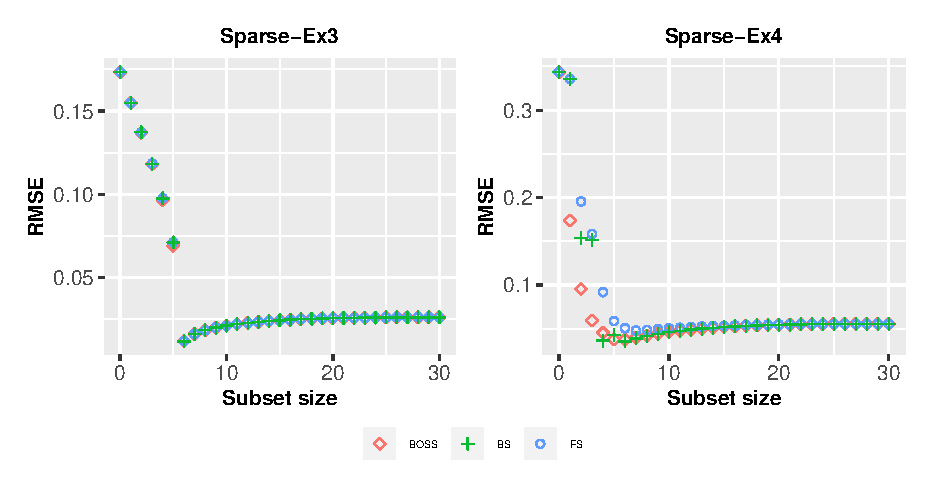
\includegraphics[width=\textwidth]{figures/rmse_solpath_lsmethods.eps}
	\caption{RMSE at each subset size, average over $1000$ replications. Note that for BOSS, the subset size $k_Q$ denotes the number of non-zero coefficients in $\hat{\gamma}(k_Q)$. In both scenarios, we have $n=200$, $p=30$, $\rho=0.9$ and high SNR.}
	\label{fig:lossratio_fs_boss_k}
\end{figure}


\subsubsection{The performance of BOSS compared to other methods}
\label{sec:boss_regu}
We now consider feasible implementations of the estimation methods. We looked at results using AICc-hdf, C$_p$-hdf and 10-fold CV for BOSS, and AICc-hdf was the best (see Supplemental Material), so that is what we will use here. For BS and FS, we will use 10-fold CV. Similar to our discussion in Section \ref{sec:bs_regu}, we find that (see Supplemental Material) AICc performs similarly to 10-fold CV for lasso, and that is what we will use for lasso. For other regularization methods, the selection rule will be 10-fold CV. According to our results (see Supplemental Material), SparseNet is slightly better than relaxed lasso and gamma lasso, and therefore we only present the results for SparseNet here. 

A selected set of simulation results is presented in Table \ref{tab:boss_regu}. Note that for BS, we only have results for $p\le 30$, since it is fitted using the ``leaps'' algorithm and $p \approx 30$ is the ad-hoc limit. We present the results in terms of $\%$ worse than the best possible BOSS, where the best possible BOSS means that on a single fit, we choose the subset size $k_Q$ with the minimum RMSE among all $p+1$ candidates, as if an oracle tells us the true model. Here is a brief summary of the results:


\begin{itemize}
	\item For BOSS, AICc-hdf has a significant advantage over CV in terms of predictive performance, except for $n=200$ and low SNR, in which case both selection rules are comparable. CV is also ten times heavier in terms of computation than AICc-hdf. These results are similar to the comparison of AICc-hdf and CV for BS with an orthogonal $X$ as discussed in Section \ref{sec:bs_ic_simulationresults}. Overall, the simulations indicate that AICc with hdf used in place of edf is a reasonable selection rule for an LS-based method that can be applied in practice without the requirement that the predictors are orthogonal. In the following discussions, when we refer to BOSS, we mean BOSS-AICc-hdf. 

	\item The performance of BOSS is comparable to the performance of BS when BS is feasible. With a small sample size $n=200$, BOSS performs either similarly to or better than BS for a high SNR, and it performs either similarly to or slightly worse than BS for a low SNR. With a large sample size $n=2000$, BOSS is generally better than BS. Furthermore, BOSS only requires fitting the procedure once while BS uses CV as the selection rule, and a single fit of BOSS only has computational cost $O(np^2)$ so that BOSS is feasible for high dimensions.

	\item The performance of BOSS is generally better than the performance of FS. In the Dense model, and Sparse-Ex3 with $n=200$ and low SNR, we see that BOSS performs similarly to FS. In all other scenarios, the advantage of BOSS is obvious. For example, in Sparse-Ex4 with $n=200$, high SNR and $\rho=0.9$, FS is almost ten times worse than BOSS in terms of RMSE. Recall that Sparse-Ex4 is an example where FS has trouble stepping in all of the true predictors (with $\beta_j \ne 0$) in early steps. This is evidenced by the fact that FS chooses eight extra predictors on average in this situation, while BOSS only chooses approximately two extra predictors. Furthermore, FS based on CV is ten times computationally heavier than BOSS. 

	\item Compared to the regularization methods, with a small sample size $n=200$, BOSS is the best when SNR is high, lasso is the best when SNR is low and SparseNet is in between. With $n=2000$, BOSS is almost always the best even when SNR is low. These findings are consistent with the discussion in Section \ref{sec:bs_regu}, where we compare the performance of BS with regularization methods under an orthogonal $X$. 

	\item In terms of support recovery in the sparse true models, LS-based methods can recover the true predictors (those with $\beta_j \ne 0$) and rarely include any noise predictors (those with $\beta_j = 0$) when SNR is high or the sample size $n$ is large. However, SparseNet and lasso generally overfit, with the latter being worse in that regard. In the low SNR and small $n$ scenario, lasso and SparseNet have more opportunity to recover the true predictors, but it comes with a price of including more false positives. 

\end{itemize}


% tab:boss_regu
% latex table generated in R 3.6.1 by xtable 1.8-4 package
% Sat Nov  9 17:57:42 2019
\begin{table}[ht]
\centering
\caption{The performance of BOSS compared to other methods. Selection rules are for 'AICc-hdf/CV' for BOSS, 
                AICc for lasso and CV for the remaining methods in the table, respectively.} 
\label{tab:boss_regu}
\scalebox{0.5}{
\begin{tabular}{|c|c|c|c|ccccc|ccccc|ccccc|}
  \toprule 
 \multicolumn{1}{|r}{} & \multicolumn{1}{r}{} & \multicolumn{1}{r}{} &       & \multicolumn{5}{c|}{Sprse-Ex3}        & \multicolumn{5}{c|}{Sparse-Ex4}       & \multicolumn{5}{c|}{Dense} \\
 \cmidrule{5-19}\multicolumn{1}{|r}{} & \multicolumn{1}{r}{} & \multicolumn{1}{r}{} &       & BOSS  & BS    & FS    & lasso & SparseNet & BOSS  & BS    & FS    & lasso & SparseNet & BOSS  & BS    & FS    & lasso & \multicolumn{1}{c|}{SparseNet}  \\
 \cmidrule{5-19}\multicolumn{1}{|c}{} & \multicolumn{1}{c}{} & \multicolumn{1}{c}{} &       & \multicolumn{15}{c|}{\% worse than the best possible BOSS}  \\
 \midrule 
 \multirow{8}[4]{*}{n=200} & \multirow{4}[2]{*}{hsnr} & \multirow{2}[1]{*}{$\rho=0.5$} & p=30 & 2/22 & 24 & 22 & 70 & 14 & 19/24 & 23 & 28 & 49 & 21 & 1/8 & 9 & 8 & 2 & 5 \\ 
   &  &  & p=180 & 1/18 & - & 21 & 135 & 17 & 4/15 & - & 16 & 82 & 13 & 14/13 & - & 16 & 47 & 8 \\ 
   &  & \multirow{2}[1]{*}{$\rho=0.9$} & p=30 & 5/41 & 17 & 41 & 66 & 12 & 21/33 & 21 & 56 & 73 & 28 & 2/9 & 10 & 8 & 2 & 8 \\ 
   &  &  & p=180 & 3/27 & - & 29 & 126 & 16 & 7/34 & - & 68 & 123 & -10 & 15/12 & - & 12 & 71 & 20 \\ 
  \cmidrule{2-19} & \multirow{4}[2]{*}{lsnr} & \multirow{2}[1]{*}{$\rho=0.5$} & p=30 & 30/25 & 25 & 25 & 0 & 7 & 35/32 & 23 & 34 & 35 & 23 & 18/17 & 16 & 18 & 10 & 11 \\ 
   &  &  & p=180 & 11/13 & - & 13 & -3 & 3 & 31/26 & - & 34 & 33 & 20 & 4/8 & - & 9 & 2 & 6 \\ 
   &  & \multirow{2}[1]{*}{$\rho=0.9$} & p=30 & 28/24 & 23 & 23 & -2 & 5 & 32/27 & 18 & 78 & 71 & 44 & 15/14 & 15 & 13 & 10 & 12 \\ 
   &  &  & p=180 & 16/16 & - & 15 & -5 & 1 & 17/18 & - & 36 & 33 & 35 & 12/10 & - & 10 & 15 & 9 \\ 
  \midrule \multirow{8}[4]{*}{n=2000} & \multirow{4}[2]{*}{hsnr} & \multirow{2}[1]{*}{$\rho=0.5$} & p=30 & 3/22 & 22 & 21 & 73 & 14 & 7/29 & 21 & 23 & 86 & 12 & 0/3 & 0 & 0 & 1 & 0 \\ 
   &  &  & p=180 & 1/22 & - & 22 & 130 & 14 & 6/28 & - & 21 & 174 & 12 & 8/9 & - & 12 & 37 & 8 \\ 
   &  & \multirow{2}[1]{*}{$\rho=0.9$} & p=30 & 2/21 & 21 & 22 & 74 & 13 & 32/33 & 16 & 33 & 108 & 12 & 0/3 & 1 & 1 & 2 & 1 \\ 
   &  &  & p=180 & 1/21 & - & 22 & 135 & 14 & 15/25 & - & 90 & 226 & 10 & 10/10 & - & 9 & 39 & 17 \\ 
  \cmidrule{2-19} & \multirow{4}[2]{*}{lsnr} & \multirow{2}[1]{*}{$\rho=0.5$} & p=30 & 5/22 & 21 & 21 & 73 & 14 & 13/30 & 22 & 23 & 61 & 15 & 2/9 & 10 & 10 & 2 & 7 \\ 
   &  &  & p=180 & 5/22 & - & 22 & 129 & 13 & 8/27 & - & 20 & 125 & 10 & 11/13 & - & 16 & 32 & 10 \\ 
   &  & \multirow{2}[1]{*}{$\rho=0.9$} & p=30 & 5/21 & 20 & 21 & 53 & 3 & 27/34 & 16 & 40 & 85 & 12 & 3/11 & 11 & 9 & 3 & 8 \\ 
   &  &  & p=180 & 4/17 & - & 17 & 92 & -5 & 14/27 & - & 104 & 179 & 20 & 12/13 & - & 11 & 40 & 18 \\ 
   \midrule 
 \multicolumn{1}{|c}{} & \multicolumn{1}{c}{} & \multicolumn{1}{c}{} &       & \multicolumn{15}{c|}{Relative efficiency} \\
 \midrule 
\multirow{8}[4]{*}{n=200} & \multirow{4}[2]{*}{hsnr} & \multirow{2}[1]{*}{$\rho=0.5$} & p=30 & 1/0.84 & 0.82 & 0.84 & 0.6 & 0.9 & 1/0.96 & 0.97 & 0.93 & 0.8 & 0.99 & 0.98/0.93 & 0.91 & 0.93 & 0.98 & 0.94 \\ 
   &  &  & p=180 & 1/0.85 & - & 0.84 & 0.43 & 0.86 & 1/0.91 & - & 0.9 & 0.57 & 0.92 & 0.95/0.96 & - & 0.93 & 0.73 & 1 \\ 
   &  & \multirow{2}[1]{*}{$\rho=0.9$} & p=30 & 1/0.74 & 0.9 & 0.74 & 0.63 & 0.93 & 1/0.91 & 1 & 0.78 & 0.7 & 0.95 & 0.98/0.91 & 0.9 & 0.92 & 0.98 & 0.93 \\ 
   &  &  & p=180 & 1/0.8 & - & 0.79 & 0.45 & 0.88 & 0.84/0.68 & - & 0.54 & 0.41 & 1 & 0.97/1 & - & 1 & 0.65 & 0.93 \\ 
  \cmidrule{2-19} & \multirow{4}[2]{*}{lsnr} & \multirow{2}[1]{*}{$\rho=0.5$} & p=30 & 0.77/0.8 & 0.8 & 0.8 & 1 & 0.93 & 0.91/0.93 & 1 & 0.92 & 0.91 & 1 & 0.93/0.94 & 0.95 & 0.93 & 1 & 0.99 \\ 
   &  &  & p=180 & 0.87/0.86 & - & 0.86 & 1 & 0.94 & 0.92/0.96 & - & 0.9 & 0.91 & 1 & 0.97/0.94 & - & 0.94 & 1 & 0.96 \\ 
   &  & \multirow{2}[1]{*}{$\rho=0.9$} & p=30 & 0.76/0.79 & 0.8 & 0.8 & 1 & 0.93 & 0.89/0.93 & 1 & 0.66 & 0.69 & 0.82 & 0.96/0.97 & 0.96 & 0.97 & 1 & 0.98 \\ 
   &  &  & p=180 & 0.82/0.82 & - & 0.83 & 1 & 0.95 & 1/0.99 & - & 0.86 & 0.88 & 0.87 & 0.97/0.99 & - & 1 & 0.95 & 1 \\ 
  \midrule \multirow{8}[4]{*}{n=2000} & \multirow{4}[2]{*}{hsnr} & \multirow{2}[1]{*}{$\rho=0.5$} & p=30 & 1/0.85 & 0.85 & 0.85 & 0.59 & 0.91 & 1/0.83 & 0.89 & 0.87 & 0.58 & 0.96 & 0.98/0.96 & 0.98 & 0.98 & 0.97 & 0.98 \\ 
   &  &  & p=180 & 1/0.83 & - & 0.83 & 0.44 & 0.89 & 1/0.83 & - & 0.88 & 0.39 & 0.95 & 1/0.99 & - & 0.96 & 0.79 & 1 \\ 
   &  & \multirow{2}[1]{*}{$\rho=0.9$} & p=30 & 1/0.84 & 0.85 & 0.84 & 0.59 & 0.9 & 0.84/0.84 & 0.96 & 0.84 & 0.54 & 1 & 1/0.97 & 0.99 & 0.99 & 0.98 & 0.99 \\ 
   &  &  & p=180 & 1/0.84 & - & 0.83 & 0.43 & 0.89 & 0.96/0.88 & - & 0.58 & 0.34 & 1 & 0.99/0.99 & - & 1 & 0.78 & 0.93 \\ 
  \cmidrule{2-19} & \multirow{4}[2]{*}{lsnr} & \multirow{2}[1]{*}{$\rho=0.5$} & p=30 & 1/0.86 & 0.86 & 0.86 & 0.61 & 0.92 & 1/0.87 & 0.93 & 0.92 & 0.7 & 0.99 & 0.98/0.91 & 0.9 & 0.91 & 0.98 & 0.93 \\ 
   &  &  & p=180 & 1/0.86 & - & 0.86 & 0.46 & 0.93 & 1/0.85 & - & 0.9 & 0.48 & 0.98 & 1/0.97 & - & 0.95 & 0.83 & 1 \\ 
   &  & \multirow{2}[1]{*}{$\rho=0.9$} & p=30 & 0.98/0.85 & 0.86 & 0.85 & 0.67 & 1 & 0.88/0.83 & 0.97 & 0.8 & 0.61 & 1 & 1/0.92 & 0.92 & 0.94 & 1 & 0.95 \\ 
   &  &  & p=180 & 0.91/0.81 & - & 0.81 & 0.49 & 1 & 1/0.9 & - & 0.56 & 0.41 & 0.95 & 0.99/0.99 & - & 1 & 0.8 & 0.94 \\ 
   \midrule 
 \multicolumn{1}{|c}{} & \multicolumn{1}{c}{} & \multicolumn{1}{c}{} &       & \multicolumn{15}{c|}{Sparsistency (number of extra variables)} \\
 \midrule 
\multirow{8}[4]{*}{n=200} & \multirow{4}[2]{*}{hsnr} & \multirow{2}[1]{*}{$\rho=0.5$} & p=30 & 6(0)/6(0.6) & 6(0.7) & 6(0.6) & 6(7.9) & 6(1.1) & 4.4(0.2)/5(1) & 5(1) & 4.8(1.1) & 5.7(10.4) & 4.8(2.1) & 29.6/26.1 & 25.1 & 26 & 29.1 & 27 \\ 
   &  &  & p=180 & 6(0)/6(0.3) & - & 6(0.4) & 6(16.6) & 6(2.4) & 4(0)/4.2(0.5) & - & 4.1(0.5) & 5.1(20.2) & 4.2(3.5) & 17/20.2 & - & 19.6 & 52.2 & 32.4 \\ 
   &  & \multirow{2}[1]{*}{$\rho=0.9$} & p=30 & 6(0.6)/6(2.1) & 6(0.8) & 6(2.1) & 6(9.2) & 6(1.6) & 5.1(2.8)/5.3(3.8) & 5(1) & 4.8(4.1) & 5.8(17.8) & 4.4(2.7) & 29.3/25.2 & 23 & 24.6 & 28.9 & 26.2 \\ 
   &  &  & p=180 & 6(0.1)/6(0.6) & - & 6(0.6) & 6(16.2) & 6(2.4) & 4.2(2.4)/4.3(4.3) & - & 4.3(8) & 4.6(44.2) & 4.1(3.1) & 15.6/21.3 & - & 17.2 & 54.4 & 37.7 \\ 
  \cmidrule{2-19} & \multirow{4}[2]{*}{lsnr} & \multirow{2}[1]{*}{$\rho=0.5$} & p=30 & 2.9(2)/3.6(2.4) & 3.4(2.1) & 3.5(2.3) & 5.1(6.9) & 4.7(5.3) & 2.3(1)/2.7(1.3) & 2.6(1) & 2.6(1.5) & 3.6(6.9) & 2.8(2.9) & 5.7/7.5 & 6.6 & 7.1 & 5.3 & 10.3 \\ 
   &  &  & p=180 & 0.3(0.1)/1(0.7) & - & 1(0.7) & 3(9.7) & 2.6(9.3) & 1(0.2)/1.6(0.9) & - & 1.3(0.8) & 2.2(10.7) & 2.1(6.5) & 0.2/1.1 & - & 0.9 & 2.7 & 6.9 \\ 
   &  & \multirow{2}[1]{*}{$\rho=0.9$} & p=30 & 1.9(2.3)/2.4(3) & 2.5(2.8) & 2.4(2.9) & 3.9(7.5) & 3.7(6.1) & 2.7(3.9)/3.2(5) & 2.7(0.9) & 2.2(4.4) & 3(10.1) & 2.9(8) & 4.1/5.2 & 4.3 & 4.5 & 8.4 & 5.9 \\ 
   &  &  & p=180 & 0.5(0.2)/1.1(1.1) & - & 1.1(1.1) & 3.2(11.1) & 3(10.8) & 0.7(1.7)/1.1(5.5) & - & 0.2(0.6) & 0.3(4.8) & 0.6(9) & 1/2.1 & - & 1.6 & 3.9 & 3.3 \\ 
  \midrule \multirow{8}[4]{*}{n=2000} & \multirow{4}[2]{*}{hsnr} & \multirow{2}[1]{*}{$\rho=0.5$} & p=30 & 6(0.1)/6(0.6) & 6(0.6) & 6(0.6) & 6(8.4) & 6(1) & 6(0.2)/6(0.6) & 6(0.6) & 6(0.6) & 6(10.9) & 6(0.8) & 30/30 & 30 & 30 & 30 & 30 \\ 
   &  &  & p=180 & 6(0)/6(0.4) & - & 6(0.4) & 6(21.5) & 6(2.3) & 6(0.1)/6(0.3) & - & 6(0.3) & 6(32.2) & 6(1.3) & 34.5/35.1 & - & 32.6 & 106.5 & 43 \\ 
   &  & \multirow{2}[1]{*}{$\rho=0.9$} & p=30 & 6(0)/6(0.6) & 6(0.6) & 6(0.6) & 6(9.2) & 6(1) & 6(0.4)/6(0.7) & 6(0.6) & 6(1.3) & 6(17.8) & 6(1.6) & 30/29.9 & 29.9 & 29.9 & 30 & 30 \\ 
   &  &  & p=180 & 6(0)/6(0.4) & - & 6(0.4) & 6(23.2) & 6(2.2) & 6(1.4)/6(1.7) & - & 5.9(3.8) & 6(72.7) & 6(8.7) & 35/38.6 & - & 30.2 & 109.6 & 52.4 \\ 
  \cmidrule{2-19} & \multirow{4}[2]{*}{lsnr} & \multirow{2}[1]{*}{$\rho=0.5$} & p=30 & 6(0.1)/6(0.6) & 6(0.6) & 6(0.6) & 6(8.3) & 6(0.7) & 4.2(0.4)/4.3(0.7) & 4.3(0.6) & 4.2(0.7) & 5.2(9.6) & 4.3(1) & 29/22.7 & 21.2 & 22.1 & 28 & 24.1 \\ 
   &  &  & p=180 & 6(0.1)/6(0.4) & - & 6(0.4) & 6(21.2) & 6(0.9) & 4(0.1)/4(0.4) & - & 4(0.4) & 4.6(26.1) & 4.1(1.3) & 16/17 & - & 14.3 & 61.8 & 25.3 \\ 
   &  & \multirow{2}[1]{*}{$\rho=0.9$} & p=30 & 5.8(0.3)/5.8(1.1) & 5.8(1.1) & 5.8(1.1) & 6(9.2) & 6(0.8) & 4.4(1.9)/4.4(1.7) & 4.3(0.6) & 4.3(2.2) & 5.4(16.6) & 4.2(2.5) & 28.8/21.2 & 18.5 & 20.2 & 27.6 & 23.5 \\ 
   &  &  & p=180 & 5.7(0.3)/5.7(0.7) & - & 5.7(0.7) & 6(23) & 6(1) & 4.1(3.6)/4.1(4.4) & - & 3.7(3.7) & 4.6(60.3) & 4.2(14.2) & 16.6/21.4 & - & 11.8 & 65.3 & 32.3 \\ 
   \bottomrule 
\end{tabular}
}
\end{table}

